\chapter{本ツールの機能}\label{cha:Function}
本研究では、帳票画像内における記入欄の座標と、その記入欄に入力する内容のデータ型をまとめたJSONファイルを出力する手法を提案する。
提案手法を実現するための手段として、まず、帳票画像内にある記入欄の位置を取得するために、記入欄を画像処理によって検出する。
次に、検出した記入欄に入力する内容のデータ型を決定するために、入力内容を示す文字を認識し、大規模言語モデルを用いて、記入する内容が、日付(date)、文字列(string)、数値(number)の3種類のうちいずれかを、ラベルとして割り付ける。

本章では、本研究で提案する手法の機能について説明する。
本ツールは、\ref{sec:input_images}節で述べた帳票画像を入力とする。
出力は、領域の座標と、対応するラベルを組とするJSON(JavaScript Object Notation)形式のファイルと、領域の座標を帳票画像に描画したPNG(Portable Network Graphics)形式の画像である。
出力する画像については、矩形の領域を描画した画像と、下線部の領域を描画した画像の2枚に分けている。
これは、領域の誤検出によって、描画した矩形と直線が重なった場合、視認性が低下することを防ぐためである。
なお、本研究で用いる用語を、表に示す。

\begin{table}[t]
	\caption{本研究で用いる用語}
	\label{tb:result_caseB_time}
	\centering
	\begin{tabular}{|c||c|}
        \hline
		用語 & 意味 \\
        \hline \hline
		帳票画像記入欄 &  入力である帳票画像内の記入欄 \\
        \hline
		電子フォーム記入欄 &  本ツールによって取得した座標で示す記入欄 \\
        \hline
		矩形領域 &  電子フォーム記入欄のうち、矩形で示された記入欄 \\
        \hline
		下線部領域 &  電子フォーム記入欄のうち、下線で示された記入欄 \\
        \hline
        領域座標 &
        \begin{tabular}{c}
            本ツールによって取得する領域の座標\\矩形領域であれば、各頂点4つののxy座標にあたる\\下線部領域であれば、両端点の2つのxy座標にあたる
        \end{tabular}\\
        \hline
        文字情報 &  
        \begin{tabular}{c}
            文字認識によって認識した文字と\\それを囲むバウンディングボックスの各頂点のxy座標
        \end{tabular}\\
        \hline
        属性 &  文字認識によって得た文字から推測するデータ型 \\
        \hline
        ラベル & 
        \begin{tabular}{c}
            文字の近傍に存在する電子フォーム記入欄に対して\\文字位置と属性から推測するデータ型
        \end{tabular}\\
        \hline
	\end{tabular}
\end{table}

また、本研究で提案する手法は、以下の2つの機能を持つ。

\begin{itemize}
    \item ラベル付き領域座標取得機能
    \item 領域描画画像出力機能
\end{itemize}

本ツールの入力対象である帳票画像の例を、図\ref{fig:original}に示す。
また、出力するJSONファイルの構造を、以下に示す。

\begin{itemize}
    \item 矩形領域のラベルと領域の座標をまとめたrects\_data配列と、下線部領域のラベルと領域座標をまとめたunderlines\_data配列がある。
    \item rects\_data配列は、以下のキーとオブジェクトから構成する。
        \begin{itemize}
            \item 取得した矩形の領域座標のうち、どの領域座標かを一意に定める番号を示すidキー
            \item 領域座標に割り付けたラベルを示すlabelキー
            \item 矩形の領域座標をまとめたcoordsオブジェクト
            \begin{itemize}
                \item 左上頂点のxy座標を示し、xキーとyキーにそれぞれx座標とy座標が対応するtop\_leftオブジェクト。
                \item 左下頂点のxy座標を示し、xキーとyキーにそれぞれx座標とy座標が対応するbottom\_leftオブジェクト。
                \item 右下頂点のxy座標を示し、xキーとyキーにそれぞれx座標とy座標が対応するbottom\_rightオブジェクト。
                \item 右上頂点のxy座標を示し、xキーとyキーにそれぞれx座標とy座標が対応するtop\_rightオブジェクト。
            \end{itemize}
        \end{itemize}
    \item underlines\_data配列は、以下のキーとオブジェクトから構成する。
        \begin{itemize}
            \item 取得した下線部の領域座標のうち、どの領域座標かを一意に定める番号を示すidキー
            \item 領域座標に割り付けたラベルを示すlabelキー
            \item 下線部の領域座標をまとめたcoordsオブジェクト
            \begin{itemize}
                \item 左端点のxy座標を示し、xキーとyキーにそれぞれx座標とy座標が対応するleftオブジェクト。
                \item 右端点のxy座標を示し、xキーとyキーにそれぞれx座標とy座標が対応するrightオブジェクト。
            \end{itemize}
        \end{itemize}
\end{itemize}

図\ref{fig:original}に対して、本ツールを適用し、出力したJSONファイルの一部を、図\ref{fig:example_output_json}に示す。

\begin{figure}[t]
    \begin{center}
        \fbox{
            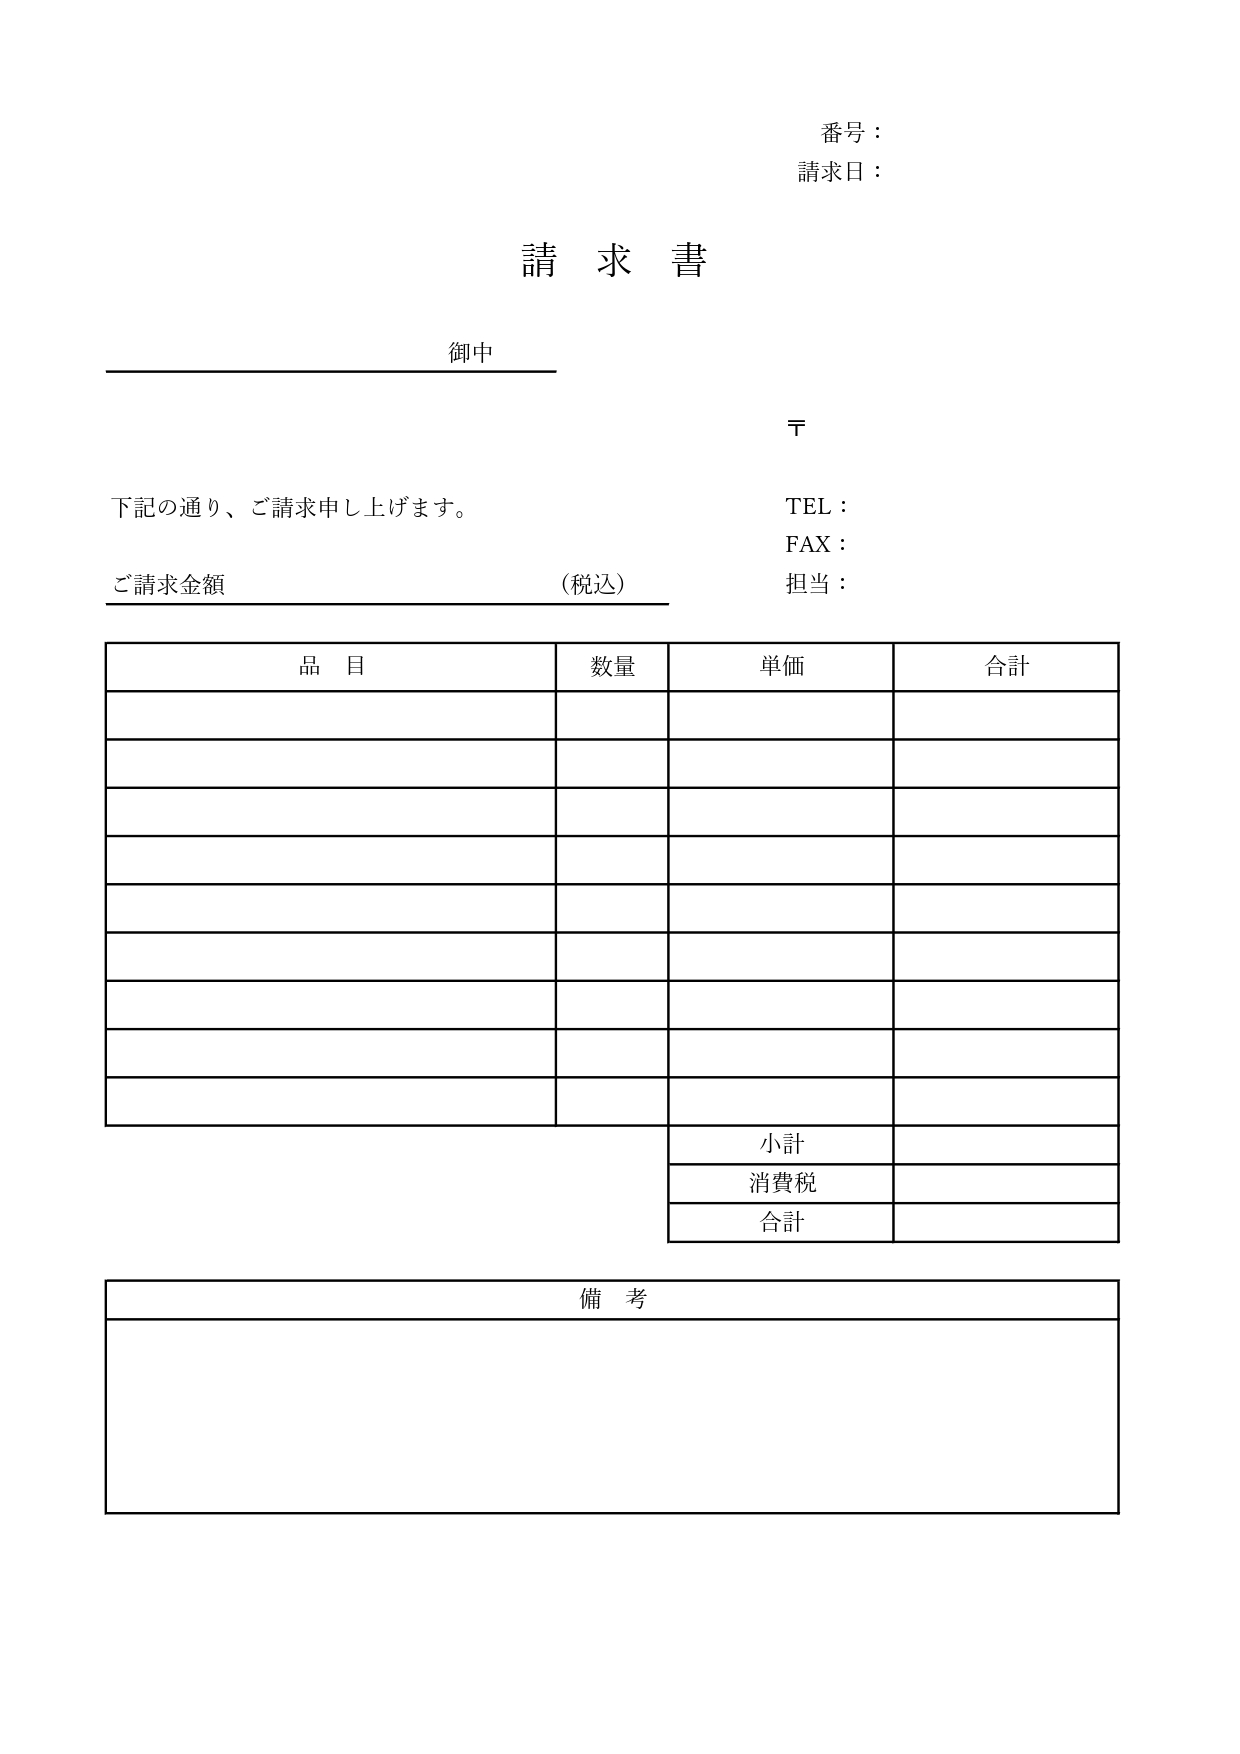
\includegraphics[width=15cm]{image/03-function/original.jpg}
        }
        \caption{入力対象である帳票画像の例}
        \label{fig:original}
    \end{center}
\end{figure}


\lstset{language=}
\begin{figure}[t]
    \begin{lstlisting}
{
    "rects_data": [
        "id": 0, 
        "label": "number",
        "coords": {
            "top_left": {
                "x": 1339,
                "y": 1288
            },
            "buttom_left": {
                "x": 1339,
                "y": 1377
            },
            "buttom_right": {
                "x": 1782,
                "y": 1377
            },
            "top_right": {
                "x": 1782,
                "y": 1288
            }
        }
    ],
    "underlines_data": [
        "id": 0,
        "label": "string",
        "coords": {
            "left": {
                "x": 213,
                "y": 742
                },
            "right": {
                "x": 1111,
                "y": 742
            }
        }
    ]
}
    \end{lstlisting}
    \caption{出力するJSONファイルの一部}\label{fig:example_output_json}
\end{figure}

\section{ラベル付き領域座標取得機能}\label{sec:eform_write_space_obtainment_feature}
ラベル付き領域座標取得機能は、取得対象の記入欄である矩形の領域および下線部の領域について、各領域の4つの座標を電子フォーム記入欄として取得する機能である。
電子フォーム記入欄にラベルを割り付けることにより、バリデーションチェック(\ref{sec:validation_check}節を参照)に必要な情報を付与することができる。

電子フォーム記入欄の取得は、以下の手順で行う。

\begin{enumerate}
    \item 矩形領域取得
    \item 下線部領域取得
    \item 文字情報取得
    \item 属性推測
    \item ラベル割付
\end{enumerate}

\subsection{矩形領域取得}\label{subsec:rect_coords_obtainment}
矩形領域取得は、矩形の領域を帳票画像記入欄とみなし、各頂点のxy座標を領域座標として取得する。
以降、下線部の領域座標と区別するため、矩形領域の領域座標を、矩形領域座標と呼ぶ。
取得した全矩形領域座標を、左上頂点のy座標を参照して昇順にソートし、0から順に番号を割り振る。
出力するJSONファイルにおける、rects\_data配列内の、割り振った番号である、idキーに対応する値を取得する。
また、rects\_data配列内の、矩形領域座標である、coordsオブジェクトのデータを取得する。

\subsection{下線部領域取得}\label{subsec:underline_coords_obtainment}
下線部領域取得は、水平な直線を帳票画像記入欄とみなし、両端点の2つのxy座標を領域座標として取得する。
以降、矩形の領域座標と区別するため、下線部領域の領域座標を、下線部領域座標と呼ぶ。
取得した全下線部領域座標を、左端点のy座標を参照して昇順にソートし、0から順に番号を割り振る。
出力するJSONファイルにおける、underlines\_data配列内の、割り振った番号である、idキーに対応する値を取得する。
また、underlines\_data配列内の、下線部領域座標である、coordsオブジェクトのデータを取得する。

\subsection{文字情報取得}\label{subsec:char_information_obtainment}
入力である帳票画像に対して文字認識を行い、検出した文字を取得文字とし、検出した文字を囲むバウンディングボックスの各頂点の座標を文字位置として、それぞれ取得する。
取得文字と文字位置は、属性推測(\ref{subsec:att_prediction}節で後述)で用いる。

\subsection{属性推測}\label{subsec:att_prediction}
取得文字に対して、大規模言語モデルによる属性の推測を行う。
本研究で用いる属性の3つの候補を、以下に示す。

\begin{itemize}
    \item 日付(date)
    \item 文字列(string)
    \item 数値(number)
\end{itemize}

以上の属性の候補から、取得文字の属性がいずれに該当するかを推測し、属性として取得する。
取得した属性は、ラベル割付(\ref{subsec:label_link}節で後述)で用いる。

\subsection{ラベル割付}\label{subsec:label_link}
\ref{subsec:rect_coords_obtainment}節と\ref{subsec:underline_coords_obtainment}節で述べた領域座標と、\ref{subsec:char_information_obtainment}節で述べた文字位置、\ref{subsec:att_prediction}節で述べた属性を用いる。
文字位置の近傍に存在する領域座標を対象に属性を割り付け、ラベルとして得る。
出力するJSONファイルにおける、rects\_data配列、およびunderlines\_data配列内の、labelキーに対応する値を取得する。

ラベル割付後、領域座標と、領域座標に対応するラベルを組としたJSONファイル(図\ref{fig:example_output_json}を参照)が、本機能の出力の1つである。


\section{領域強調画像出力機能}\label{sec:highlighted_area_image_output}
領域強調画像出力機能は、入力である帳票画像に対して、取得した領域座標とラベルを描画することによって、強調表示したPNG画像を出力する機能である。
これによって、\ref{sec:eform_write_space_obtainment_feature}節で述べた、ラベル付き領域座標取得機能で出力したJSONファイルの内容を、目視で確認しやすくなる。
本機能で出力する画像は、矩形領域を強調した矩形領域強調画像と、下線部領域を強調した下線部領域強調画像の計2枚である。
矩形領域強調画像は、ランダムなRGBカラーで矩形を描画し、下線部領域強調画像は、緑色で直線を描画する。
矩形をランダムなRGBカラーで描画する理由は、矩形領域が隣接する際に、視認性が低下することを防ぐためである。

図\ref{fig:original}に示した帳票画像記入欄のうち、矩形の帳票画像記入欄の一部を切り取った画像を、図\ref{fig:rect_original}に示す。
また、図\ref{fig:rect_original}の画像に対し、本機能を適用した画像を、図\ref{fig:rect_drawing}に示す。
図\ref{fig:rect_drawing}の画像から、矩形領域座標を参照してランダムなRGBカラーで矩形を描画し、同色で矩形左上に番号と文字列を表示していることがわかる。
図\ref{fig:rect_drawing}の矩形に表示する番号は、JSONファイル内のrect\_data配列のidキーに対応する値と一致する。
同様に、番号の右に表示する文字列は、JSONファイル内のrects\_data配列のlabelキーに対応する値と一致する。
図\ref{fig:rect_drawing}の画像中にある、「単価」という文字がある矩形の左上頂点には、「0: number」と描画している。
これは、rects\_data配列のidキーに0が、labelキーにnumberがそれぞれ対応することを示す。

\begin{figure}[t]
    \begin{center}
        \fbox{
            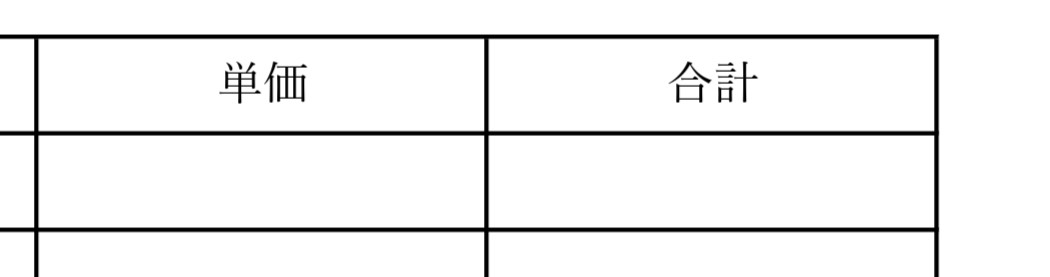
\includegraphics[width=15cm]{image/03-function/rect_original.jpg}
        }
        \caption{帳票画像にある矩形の記入欄}
        \label{fig:rect_original}
    \end{center}
\end{figure}

\begin{figure}[t]
    \begin{center}
        \fbox{
            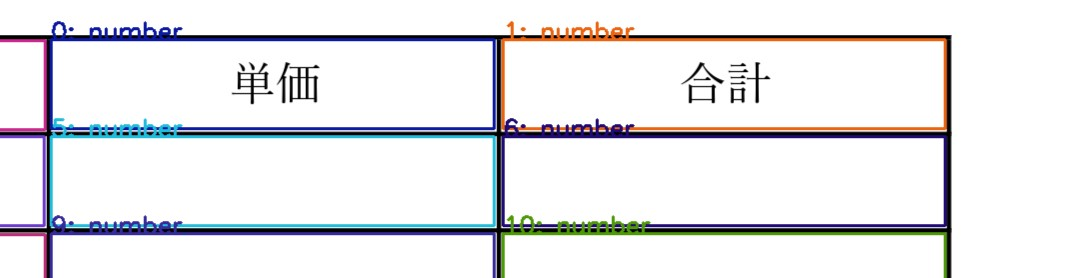
\includegraphics[width=15cm]{image/03-function/rects_with_label.jpg}
        }
        \caption{取得した矩形領域座標の描画}
        \label{fig:rect_drawing}
    \end{center}
\end{figure}

図\ref{fig:original}内にある帳票画像記入欄のうち、下線部帳票画像記入欄を切り取った画像を、図\ref{fig:underline_original}に示す。
また、図\ref{fig:underline_original}の画像に対し、下線部領域座標とラベルを取得し、描画した画像を、図\ref{fig:underline_drawing}に示す。
図\ref{fig:underline_drawing}の画像から、下線部領域座標を参照して緑色で直線を描画し、同色で直線の左端点に番号と文字列を表示していることがわかる。
図\ref{fig:underline_drawing}の下線部に表示する番号は、JSONファイル内のunderlines\_data配列のidキーに対応する値と一致する。
同様に、番号の右に表示する文字列は、JSONファイル内のunderlines\_data配列のlabelキーに対応する値と一致する。
図\ref{fig:rect_drawing}の画像中にある、「御中」という文字の左にある下線部の左端点には、「0: number」と描画している。
これは、underlines\_data配列のidキーに0が、labelキーにstringがそれぞれ対応することを示す。

\begin{figure}[t]
    \begin{center}
        \fbox{
            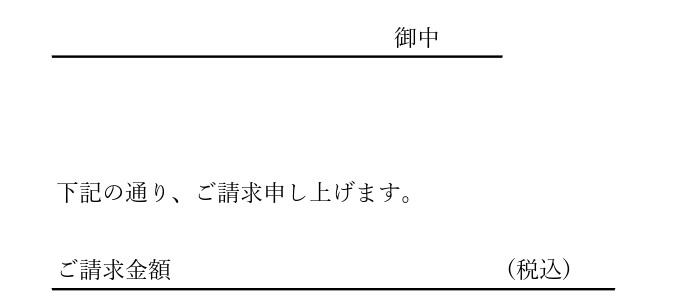
\includegraphics[width=15cm]{image/03-function/underline_original.jpg}
        }
        \caption{帳票画像にある下線部の記入欄}
        \label{fig:underline_original}
    \end{center}
\end{figure}

\begin{figure}[t]
    \begin{center}
        \fbox{
            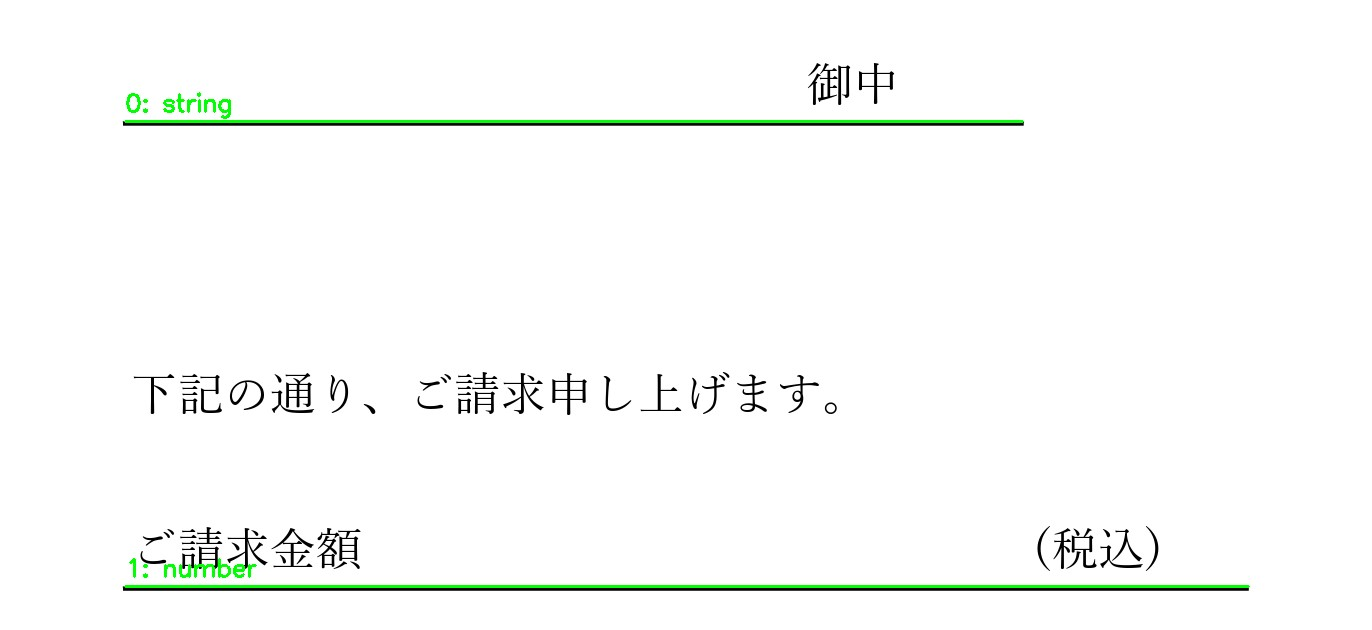
\includegraphics[width=15cm]{image/03-function/underlines_with_label.jpg}
        }
        \caption{取得した下線部領域座標の描画}
        \label{fig:underline_drawing}
    \end{center}
\end{figure}

入力である帳票画像に対して、矩形領域座標とラベルを描画した画像(図\ref{fig:rect_drawing}を参照)と、下線部領域座標とラベルを描画した画像(図\ref{fig:underline_drawing}を参照)の2つのPNG画像が、本機能の出力の1つである。